
%This is the segment that can be as long or short as needed to finish in time. Leave to end.
%Performance Analysis. Discuss impact of number of planes, size of planes, etc, with collected data. Highlight areas of improvement, engineering challenges with memory usage, reuse of buffers, reduction of memory usage by parameter tweaking, stream overlapping. Try to benchmark against other algorithms if have time, but probably won't.
\chapter{Results and Analysis}
\label{chap:analysis}
This chapter provides some example results from the finished pipeline as well as some performance analysis. The runtime of some stages of the pipeline is heavily dependent on the target scene complexity. All measurements in this chapter were performed on a workstation with an Intel i5-3570K CPU @3.40GHz, 8.00 GB of RAM, Windows 8.1 64-bit, and a GeForce GTX 760 GPU. \par 

\section{Results}
The pipeline is tuned to look for large planar surfaces like walls, furniture, ceilings, and floors. Figure~\ref{fig:uppercorner} shows an example of a high quality segmentation result. The mesh reconstruction is visualized in the lower left corner through a virtual camera with the same intrinsic parameters as the original sensor for direct comparison. In this image, almost the entire scene is composed of planes, so the reconstruction is nearly complete.\par 
Because the Kinect is based on structured infrared light, the result is robust to varying lighting conditions. Figure~\ref{fig:uppercornerwireframelowlight} shows a darker version of the same scene with the QuadTree mesh overlaid in green.
\subsection{Successes}
\begin{figure}[!htpb]
    \centering
    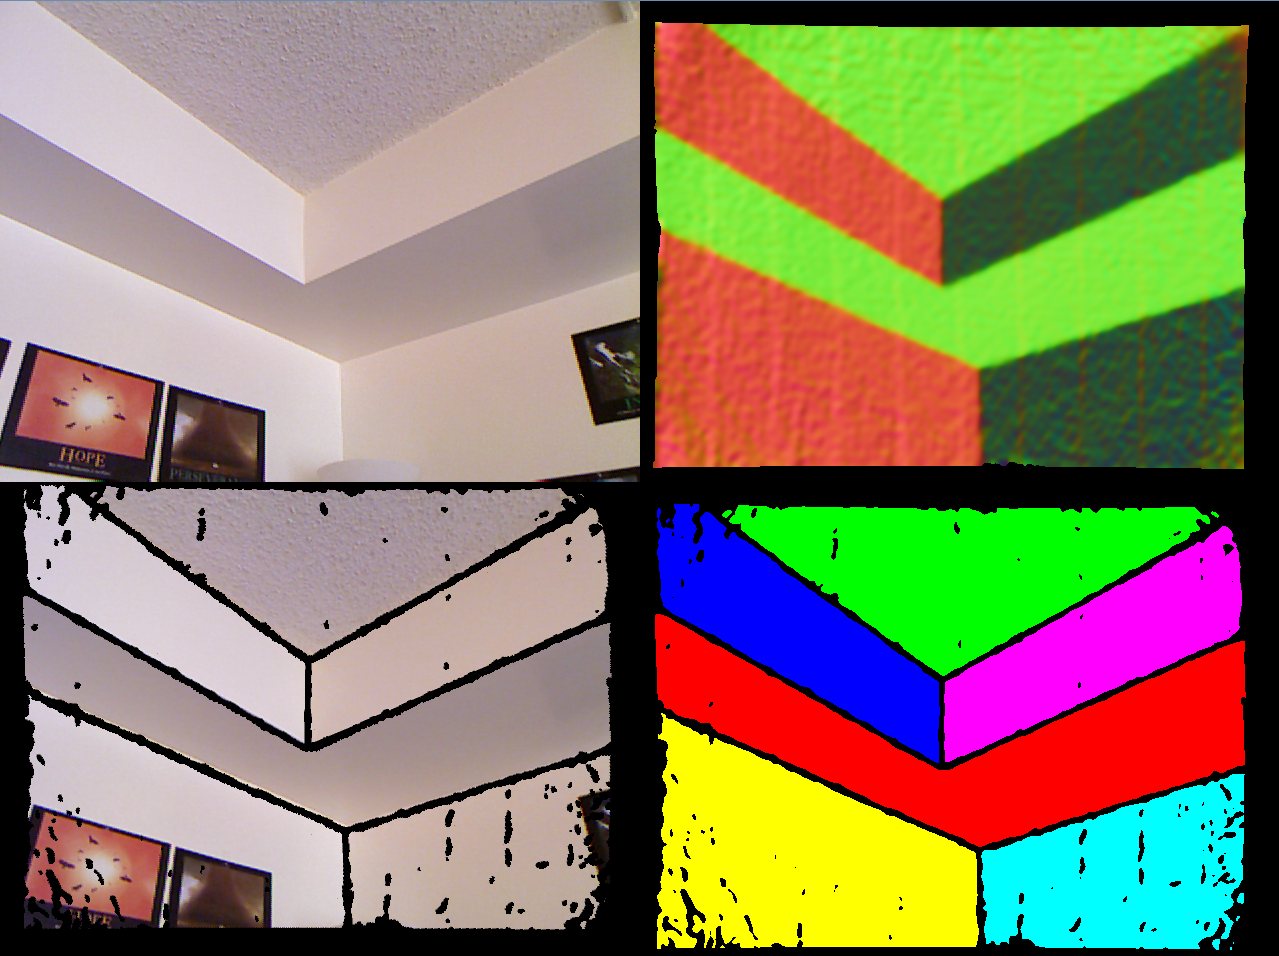
\includegraphics[width=0.8\textwidth]{UpperCornerResults.png}
    \caption{Example results of the upper corner of a room, 3 sets of 2 parallel planes detected.  Upper-left) original color image. Upper-right) surface normal estimates. Lower-left) mesh reconstruction. Lower-right) Random colorization of plane segments}
    \label{fig:uppercorner}
\end{figure}

\begin{figure}[!htpb]
    \centering
    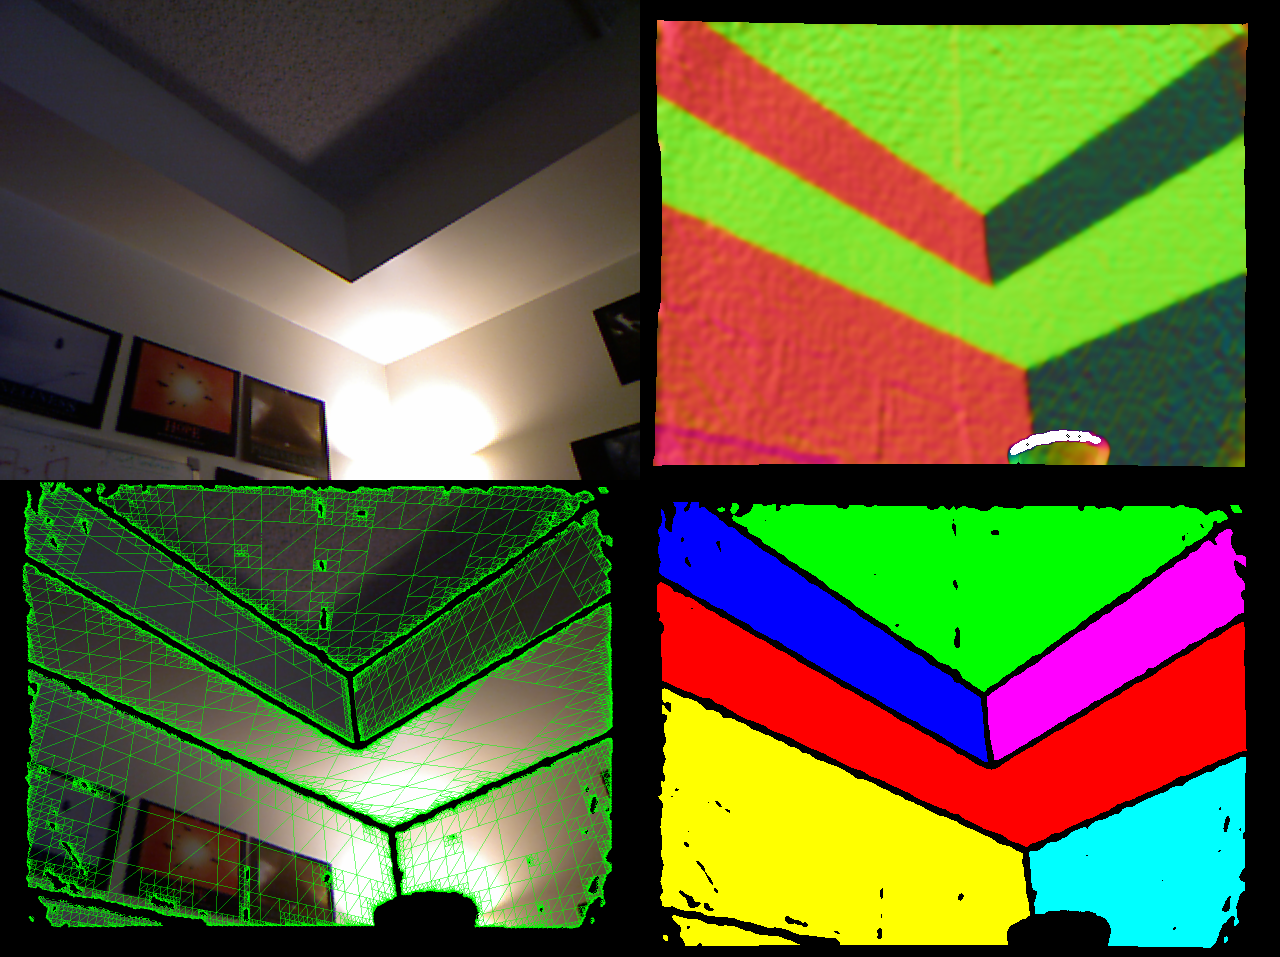
\includegraphics[width=0.8\textwidth]{UpperCornerResultsWireframe.png}
    \caption{Example results of the upper corner of a room in low light conditions with wireframe.  Upper-left) original color image. Upper-right) surface normal estimates. Lower-left) mesh reconstruction. Lower-right) Random colorization of plane segments}
    \label{fig:uppercornerwireframelowlight}
\end{figure}
As it turns out, the pipeline is very good at floor plane detection. Figure~\ref{fig:floorplane} shows a reconstruction of an empty lab floor with a tape soccer field pattern. Because the algorithm is looking for global plane solutions, the result is very robust to occlusion (Figures~\ref{fig:meshoutput} and ~\ref{fig:naoquadtree}). These images also demonstrate how adaptable the QuadTree representation is. Note that around the hole left by the robot in Figure~\ref{fig:naoquadtree} the QuadTree almost perfectly reconstructs the silhouette almost perfectly.

\begin{figure}[!htpb]
    \centering
    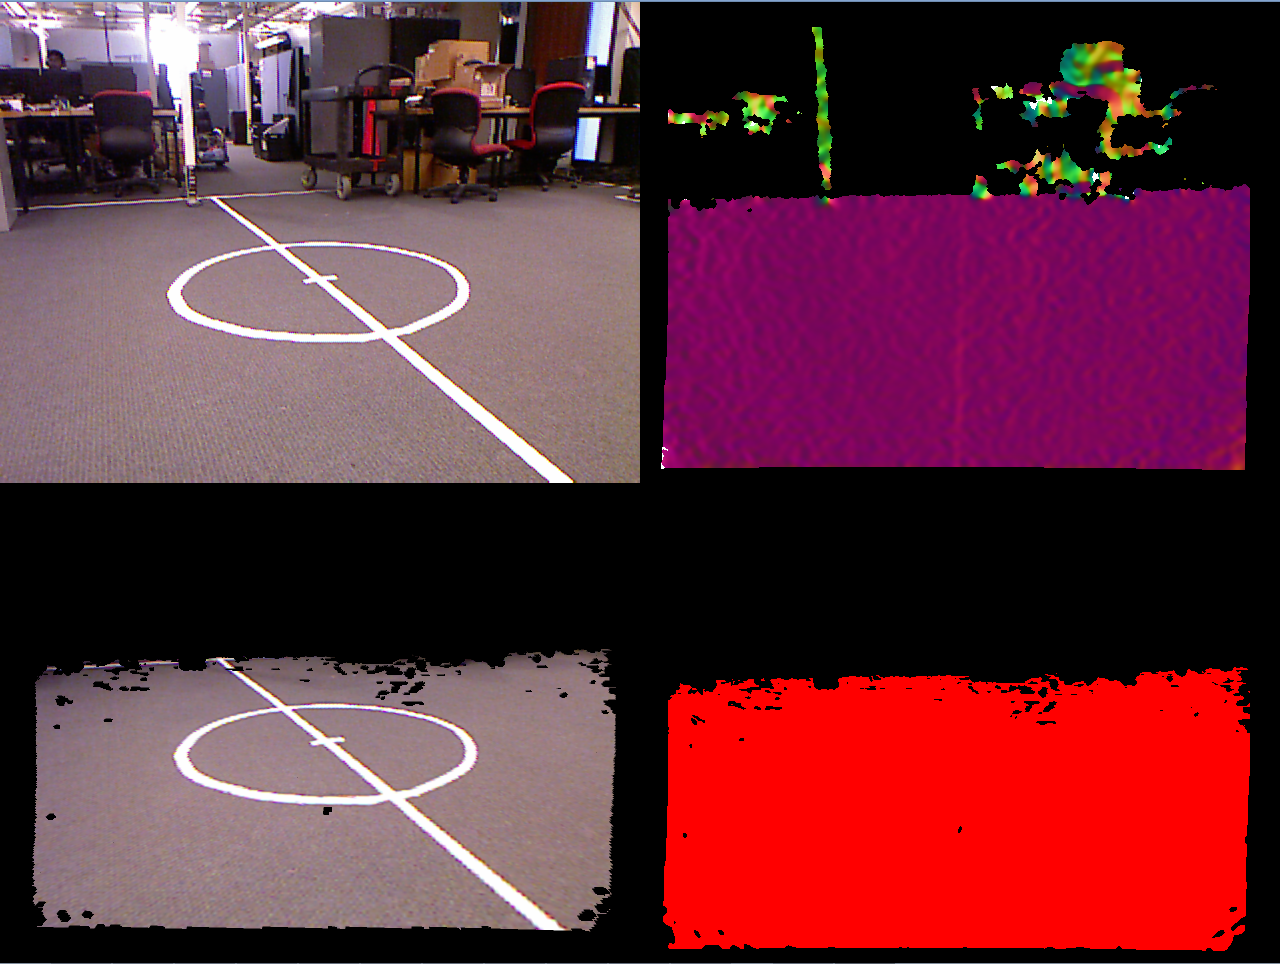
\includegraphics[width=0.8\textwidth]{EmptyGraspFieldResults.png}
    \caption{Effortless floor plane detection. Upper-left) original color image. Upper-right) surface normal estimates. Lower-left) mesh reconstruction. Lower-right) Random colorization of plane segments}
    \label{fig:floorplane}
\end{figure}


\begin{figure}[!htpb]
    \centering
    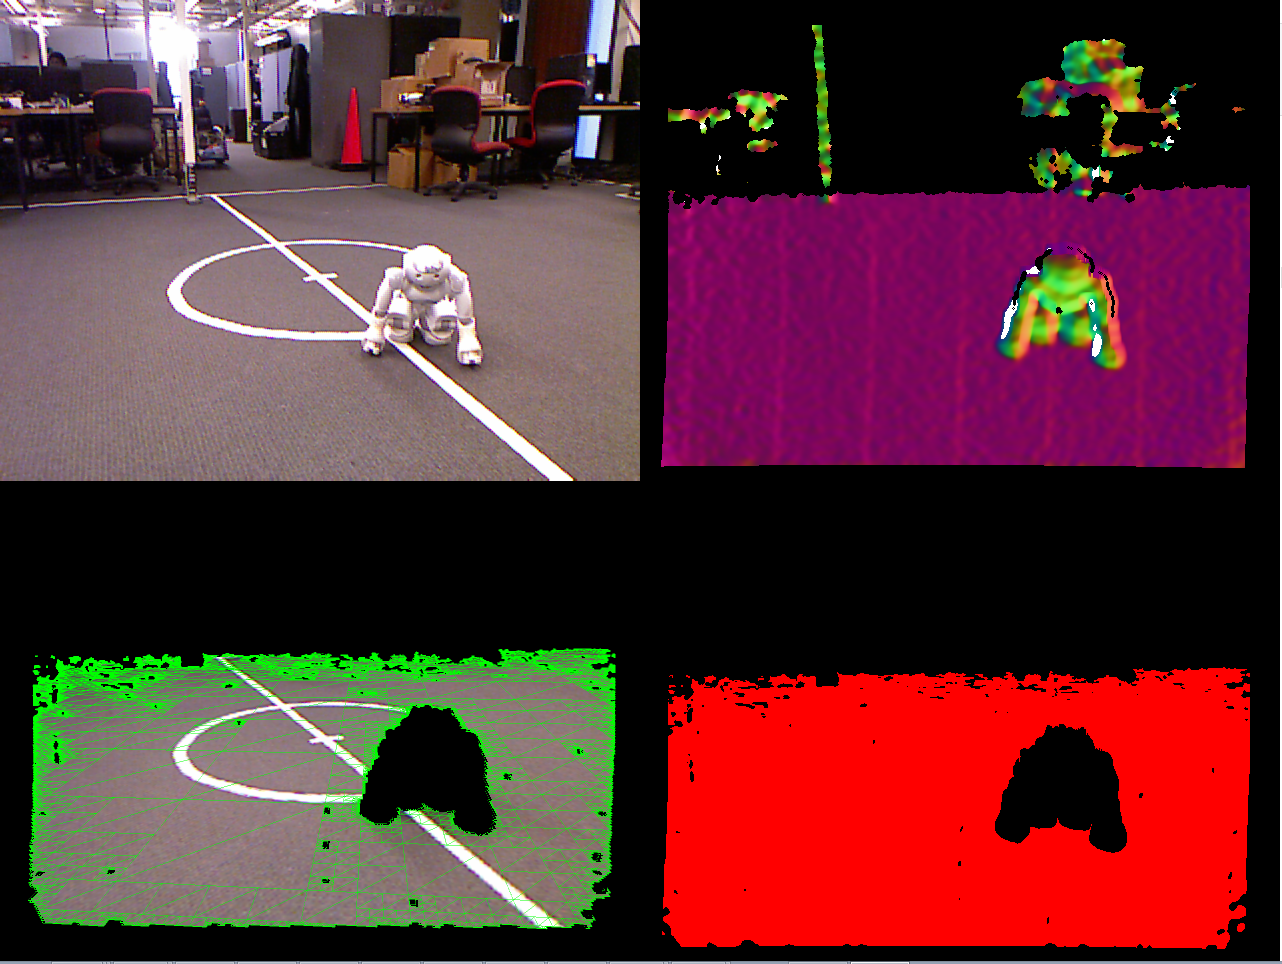
\includegraphics[width=0.8\textwidth]{NaoGraspFieldResults.png}
    \caption{Lab floor with small obstruction to demonstrate QuadTree flexibility. Upper-left) original color image. Upper-right) surface normal estimates. Lower-left) mesh reconstruction. Lower-right) Random colorization of plane segments}
    \label{fig:naoquadtree}
\end{figure}


\subsection{Failures}
However, the pipeline does have several issues and common failure cases. Figure~\ref{fig:foamboxes} shows an example of pseudo-planar surfaces that are partially detected. Because the box sides are multifaceted, the algorithm detects a broken surface, if it detects the surface at all. A more serious issue is shallowly curved surfaces like lampshades or large building columns are sometimes detected as a series of small plane segments as in Figure~\ref{fig:lampcurve}. Not only does this represent a false positive on a clearly non-planar surfaces, but it also creates a set of false planes that can cause segmentation errors in other parts of the scene.

\begin{figure}[!htpb]
    \centering
    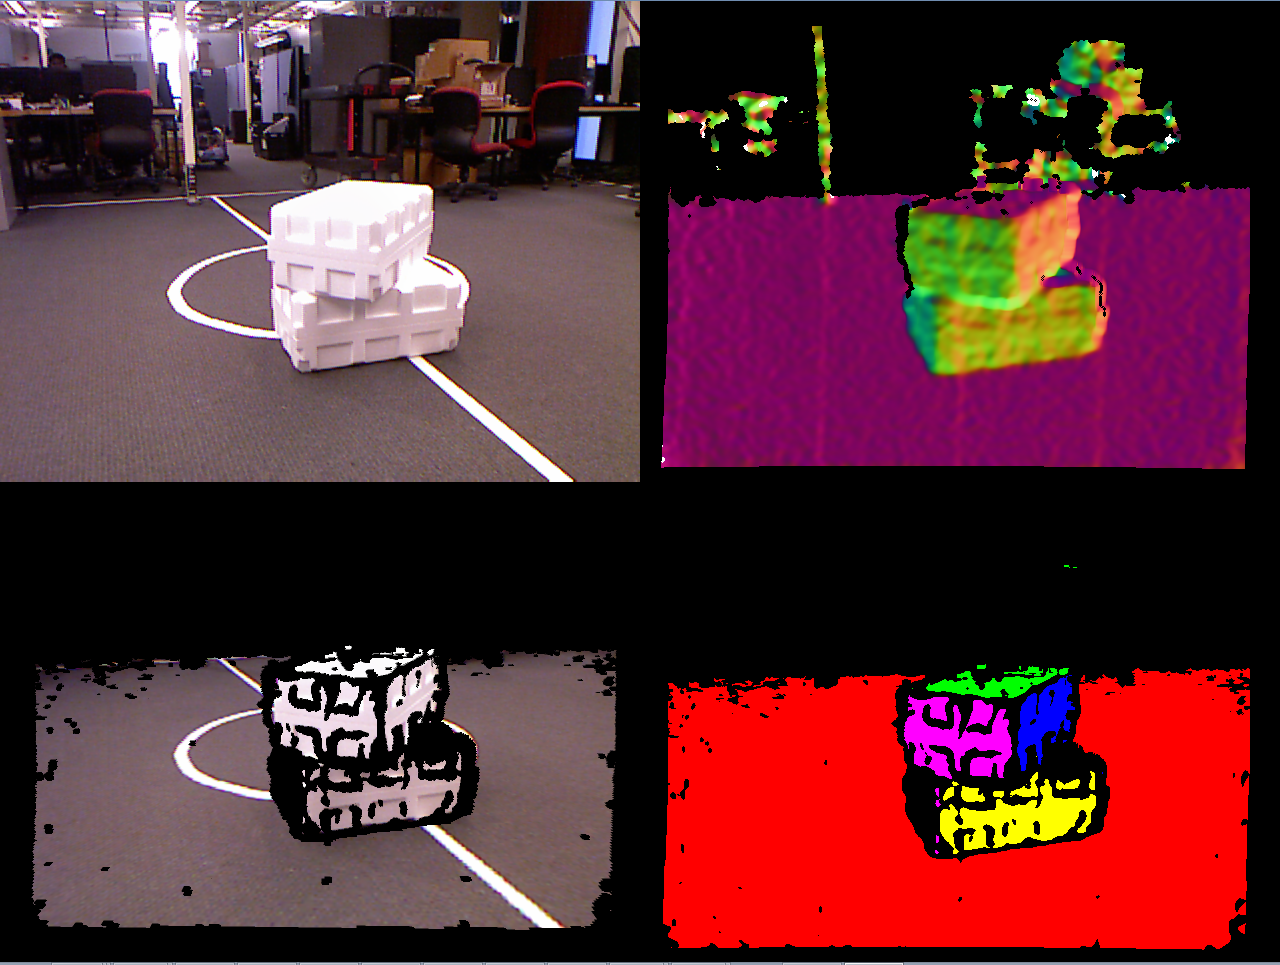
\includegraphics[width=0.8\textwidth]{FoamBoxesResults.png}
    \caption{Algorithm has difficulty with pseudo-planar surfaces. Upper-left) original color image. Upper-right) surface normal estimates. Lower-left) mesh reconstruction. Lower-right) Random colorization of plane segments}
    \label{fig:foamboxes}
\end{figure}

\begin{figure}[!htpb]
    \centering
    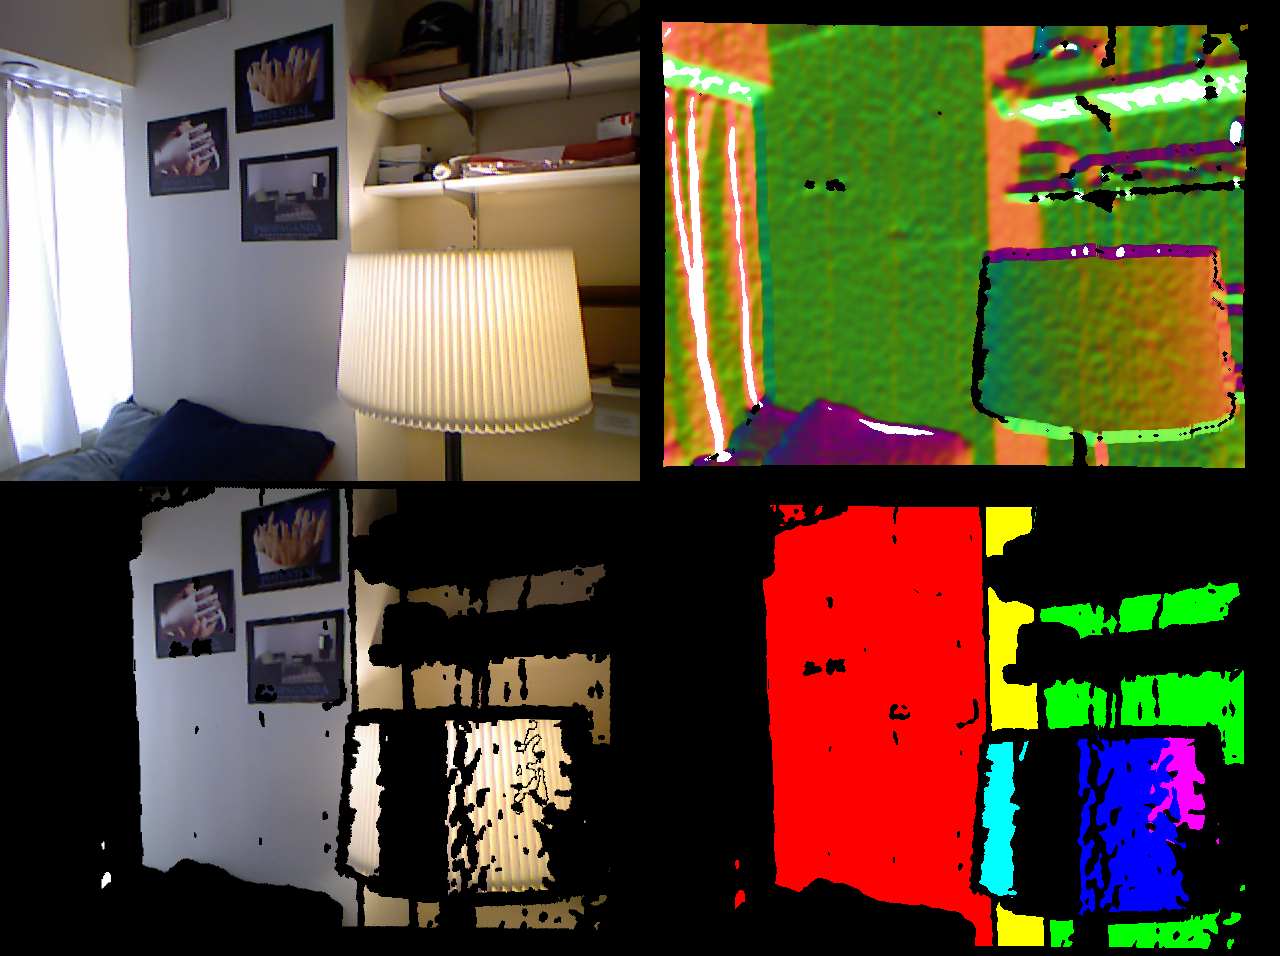
\includegraphics[width=0.8\textwidth]{LampFailureResults.png}
    \caption{Algorithm incorrectly detects large smooth curves as multiple planes. Upper-left) original color image. Upper-right) surface normal estimates. Lower-left) mesh reconstruction. Lower-right) Random colorization of plane segments}
    \label{fig:lampcurve}
\end{figure}

Figure~\ref{fig:distantsmallplane} shows an object that is clearly a plane 2.5 meters from the sensor that is only partially detected due to noise and decreased resolution. This is likely because the segmentation thresholds are constant across the full range of sensor accuracy and resolution, so surfaces at the extreme of the sensor's usable range are very likely to be broken up or poorly segmented. Adding resolution dependent thresholds is not a trivial task, because large planes can vary in resolution greatly from end to end.

\begin{figure}[!htpb]
    \centering
    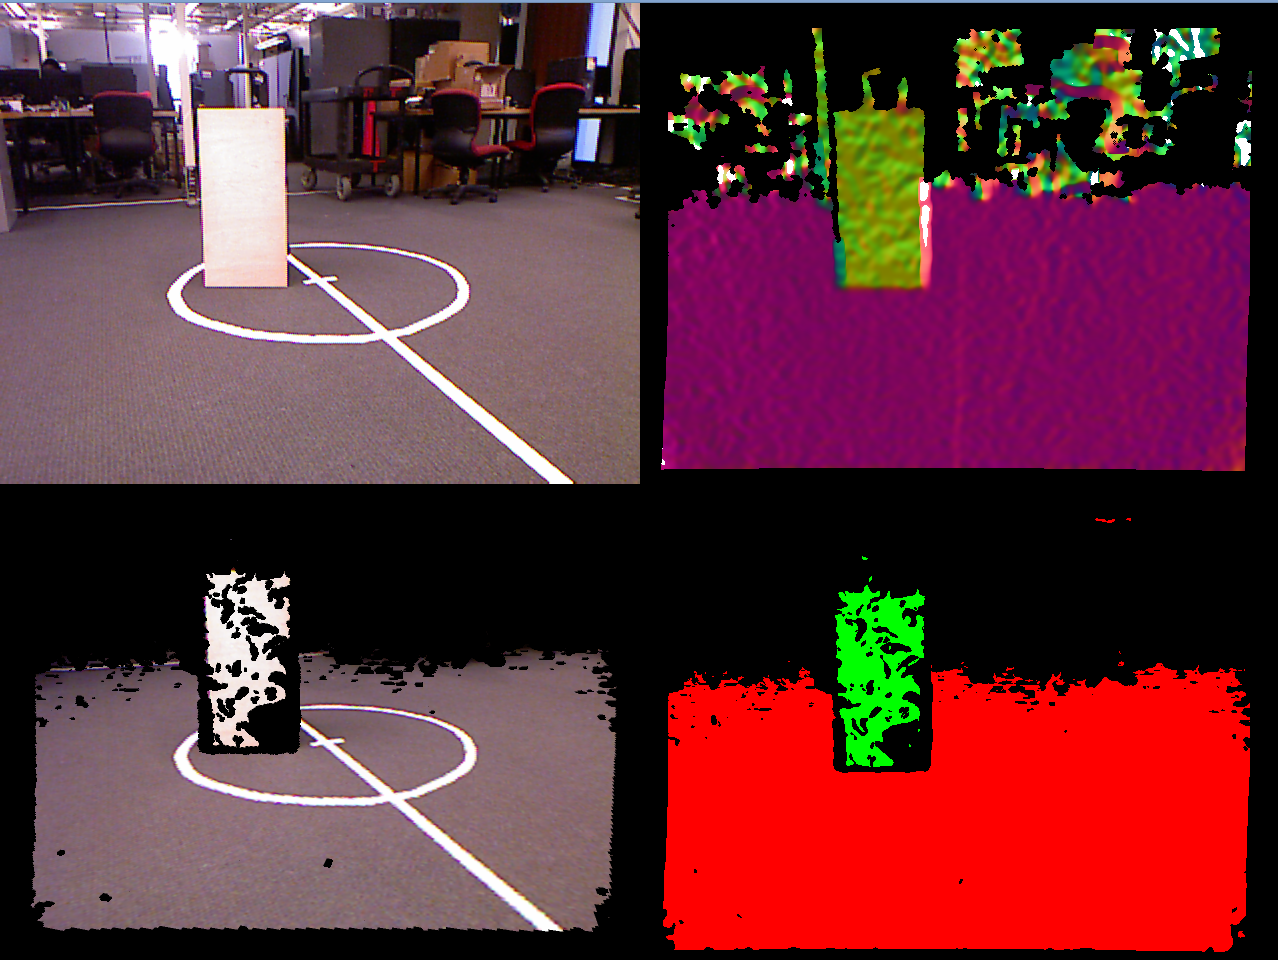
\includegraphics[width=0.8\textwidth]{BoardAndBoxResults.png}
    \caption{Fails to cleanly detect obvious plane 2.5m away. Upper-left) original color image. Upper-right) surface normal estimates. Lower-left) mesh reconstruction. Lower-right) Random colorization of plane segments}
    \label{fig:distantsmallplane}
\end{figure}

Figure~\ref{fig:missingwall} demonstrates a failing of the simple segmentation system I developed. If two large planes in the image (the wall and the whiteboard in this case) are very close to being parallel with each other, sometimes one of the planes will be completely missed. Also, when these closely related planes intersect, as is also the case in this image, an area tracing the plane intersection can be mislabeled. This is represented in Figure~\ref{fig:missingwall} by the horizontal strip of red spots extending from the upper right corner of the whiteboard segment extending towards the floorlamp. The plane intersection problem also shows up even when both planes are correctly detected (Figure~\ref{fig:planeintersect}).


\begin{figure}[!htpb]
    \centering
    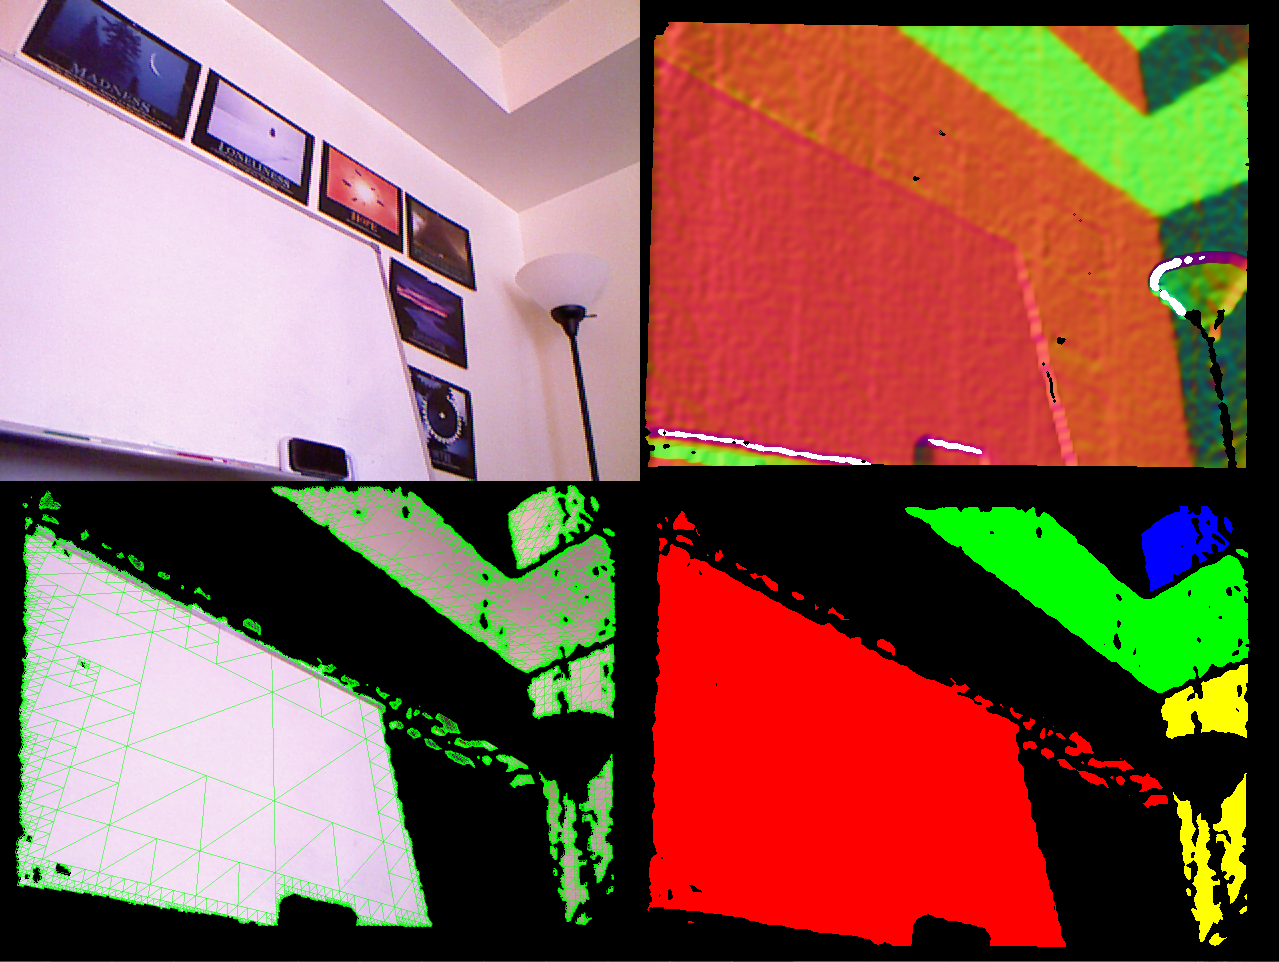
\includegraphics[width=0.8\textwidth]{MissingWall.png}
    \caption{Two planes with similar normals, only one is detected. Upper-left) original color image. Upper-right) surface normal estimates. Lower-left) mesh reconstruction. Lower-right) Random colorization of plane segments}
    \label{fig:missingwall}
\end{figure}



\begin{figure}[!htpb]
    \centering
    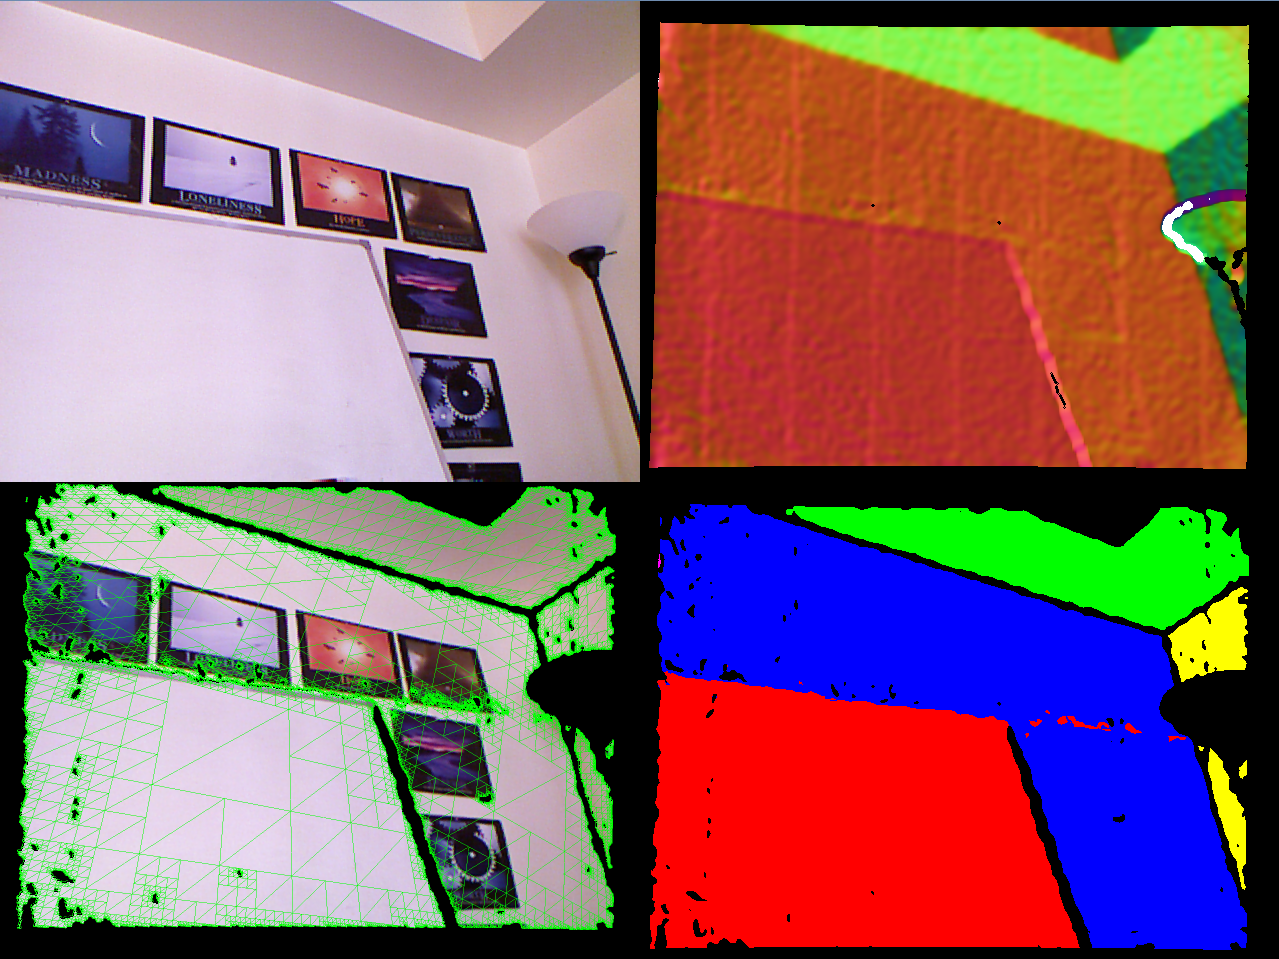
\includegraphics[width=1.0\textwidth]{PlaneIntersection.png}
    \caption{Two nearly parallel planes that intersect show some segmentation errors. Upper-left) original color image. Upper-right) surface normal estimates. Lower-left) mesh reconstruction. Lower-right) Random colorization of plane segments}
    \label{fig:planeintersect}
\end{figure}



\section{Performance Analysis}
\subsection{Runtime Analysis}
One of the primary goals of this thesis is to ensure that the pipeline runs in near realtime. For a frame rate of roughly 30FPS, the entire pipeline must run in less than 32ms per frame. Most of the pipeline was designed to  have roughly the same runtime regardless of the scene being imaged. However, some segments of the pipeline are heavily data dependent. In particular, the number of planes detected in the image has a huge impact on the runtime of the mesh generation module.\par 

Figure~\ref{fig:runtimebystage} shows the runtime of each major pipeline module outlined in Chapter~\ref{chap:implementation} based data collected on a variety of scenes (n=2541). The memory management section has not been previously discussed and is responsible for deleting the results of the previous iteration. 

\begin{figure}[!htpb]
    \centering
    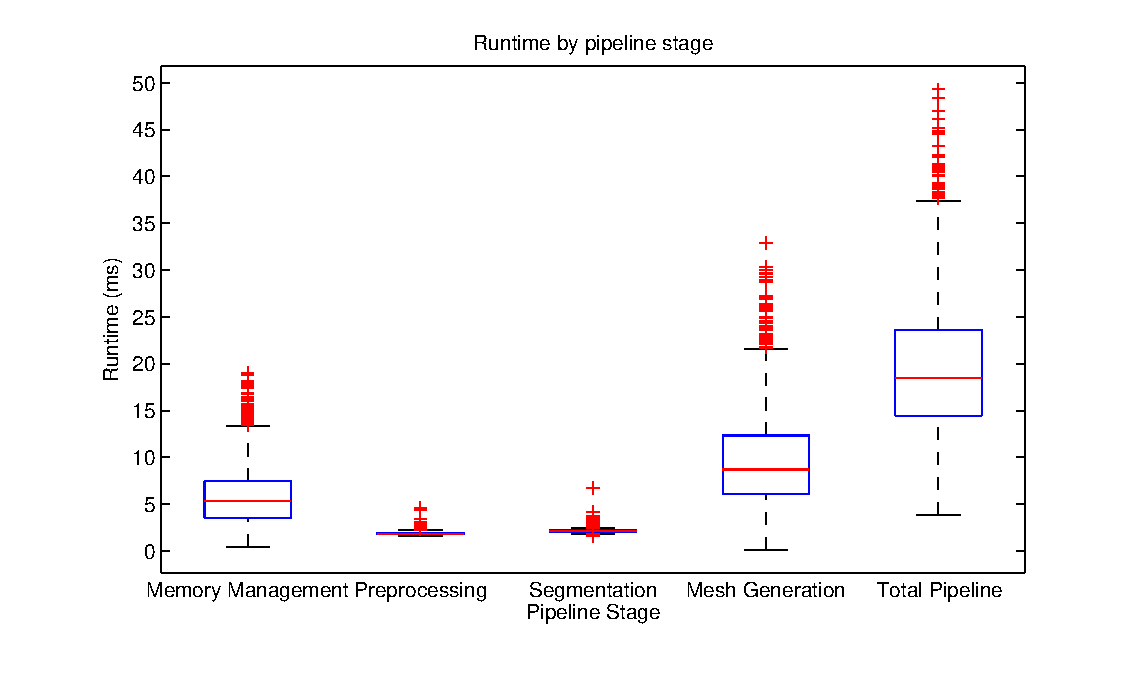
\includegraphics[width=1.0\textwidth]{RuntimeByPipelineStage.eps}
    \caption{Pipeline runtime broken down by stage.}
    \label{fig:runtimebystage}
\end{figure}

Note that both the preprocessing and segementation stages have very consistent runtimes with medians of 1.83 ms and 2.13 ms respectively. Figures~\ref{fig:preprocessingplanes} and ~\ref{fig:segementationplanes} show that apart from the case where no planes were detected, the number of planes in the image had practically no effect on either stage's runtime. However, the mesh generation stage varies greatly in runtime. Figure~\ref{fig:meshgenerationplanes} clearly demonstrates a positive correlation between the number of planes detected  and the total runtime of the stage. Likewise, the memory management stage shows a slight increase in runtime as the number of planes increases.\par

\begin{figure}[!htpb]
    \centering
    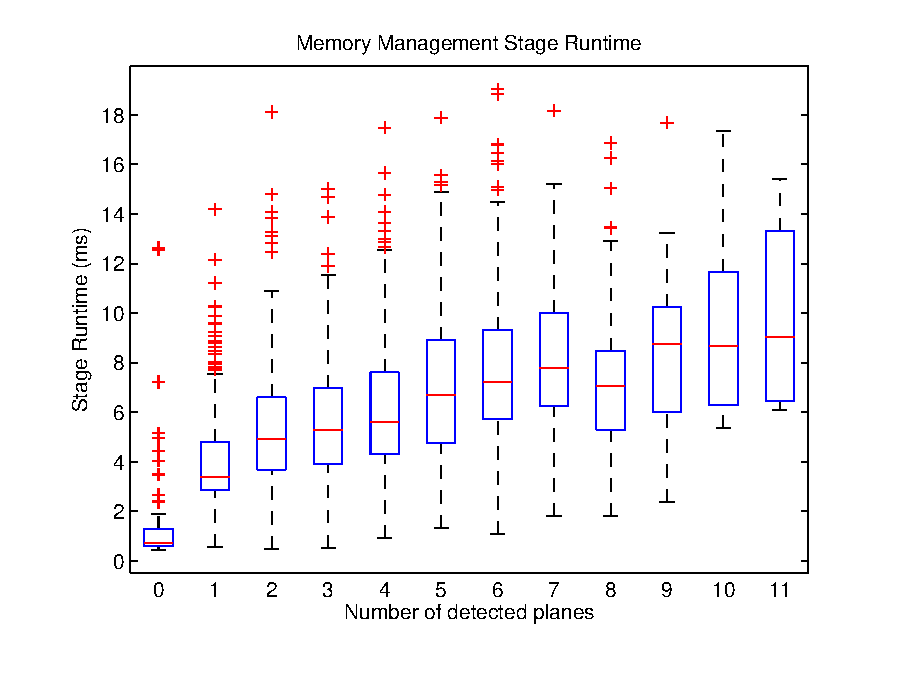
\includegraphics[width=0.7\textwidth]{MemoryManagementByNumPlanes.eps}
    \caption{Runtime of the memory management stage by number of detected planes.}
    \label{fig:memorymangementplanes}
\end{figure}


\begin{figure}[!htpb]
    \centering
    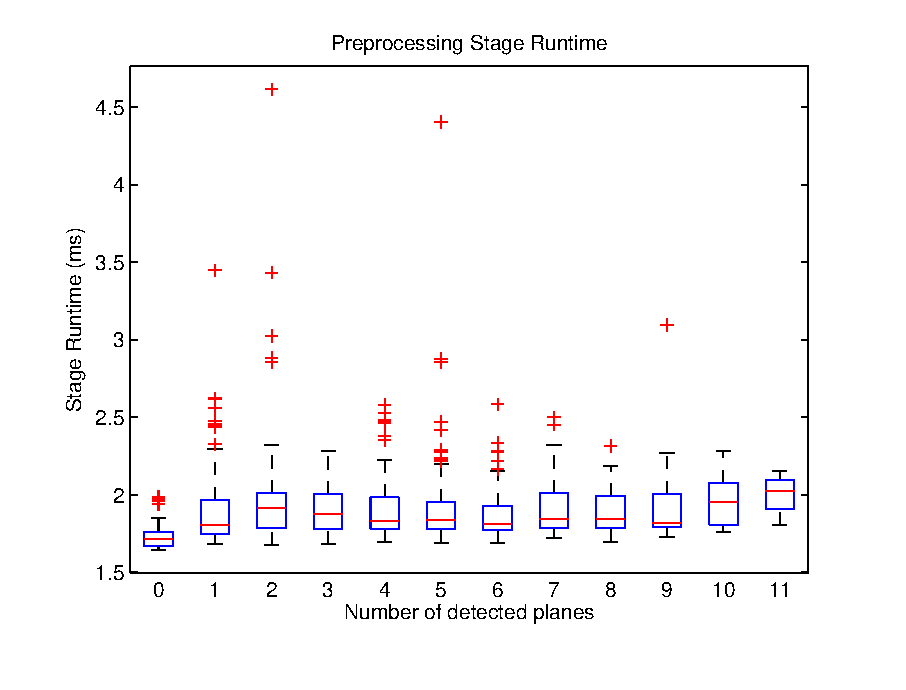
\includegraphics[width=0.7\textwidth]{PreprocessingByNumPlanes.eps}
    \caption{Runtime of the preprocessing stage by number of detected planes.}
    \label{fig:preprocessingplanes}
\end{figure}



\begin{figure}[!htpb]
    \centering
    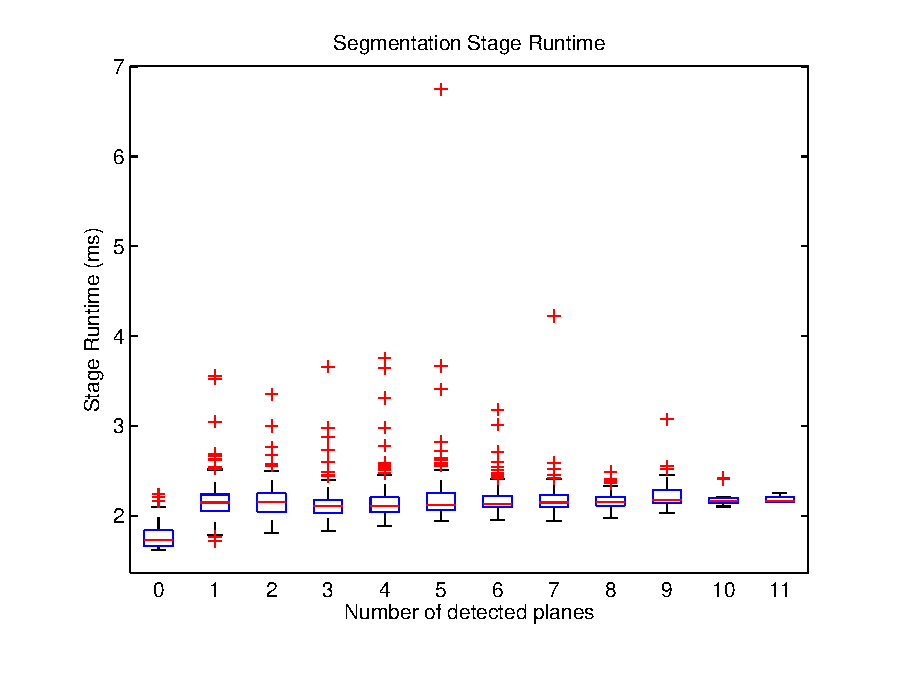
\includegraphics[width=0.7\textwidth]{SegmentationByNumPlanes.eps}
    \caption{Runtime of the segmentation stage by number of detected planes.}
    \label{fig:segementationplanes}
\end{figure}



\begin{figure}[!htpb]
    \centering
    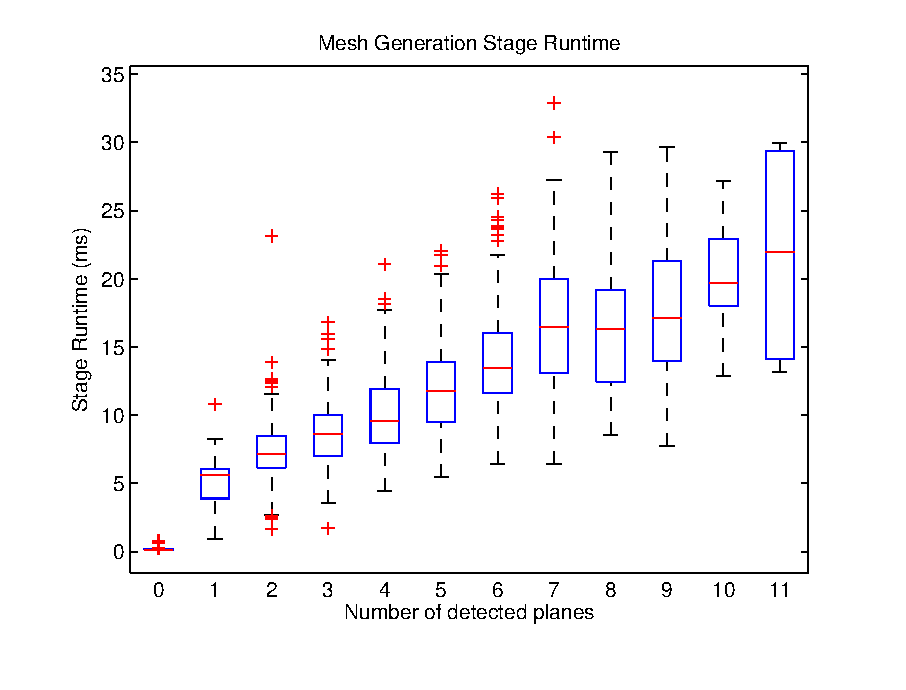
\includegraphics[width=0.7\textwidth]{MeshGenerationByNumPlanes.eps}
    \caption{Runtime of the mesh generation stage by number of detected planes.}
    \label{fig:meshgenerationplanes}
\end{figure}

How has this affected the ability of the system to run in real-time? Figure~\ref{fig:pipelineplanes} shows the total pipeline runtime for varying number of detected planes. The pipeline reliably achieves real-time performance when less than 6 planes are detected, and continues to achieve near real-time performance up to the most complicated scene with 11 planes.

\begin{figure}[!htpb]
    \centering
    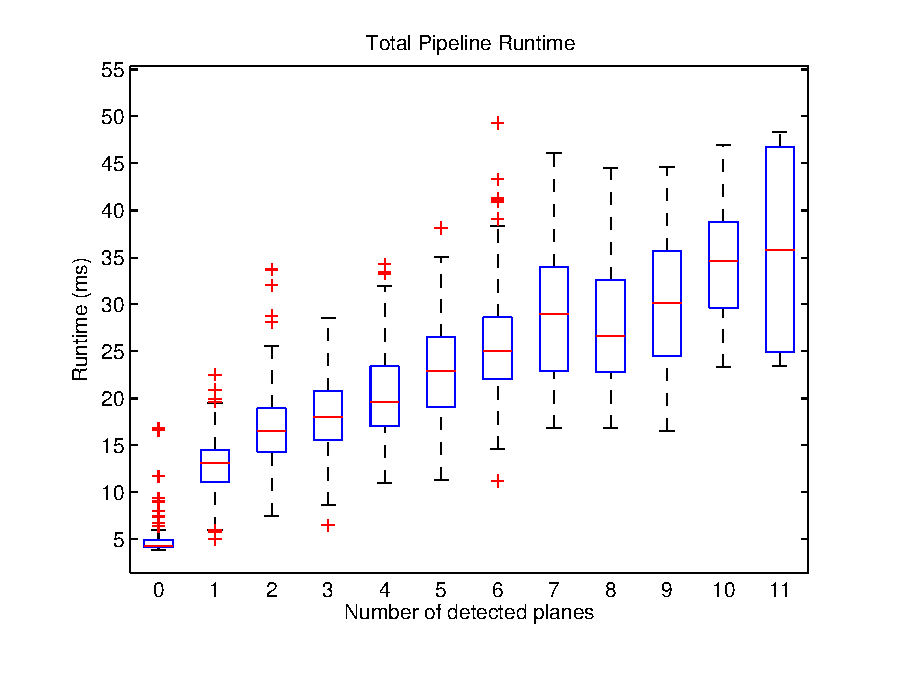
\includegraphics[width=0.7\textwidth]{PipelineByNumPlanes.eps}
    \caption{Runtime of the entire pipeline by number of detected planes.}
    \label{fig:pipelineplanes}
\end{figure}


\subsection{Timeline Breakdown}
The compute timeline of the pipeline is shown in Figure~\ref{fig:fulltimeline}. This view of the pipeline helps identify some key areas of the pipeline that could benefit from optimization. The GPU is idle for the vast majority of the memory management section of the timeline, during which the CPU performs memory cleanup tasks.  These tasks could be run in parallel with the next two pipeline stages, saving approximately 3ms per run.\par
The preprocessing timeline (Figure~\ref{fig:preprocessingtimeline}) shows a significant gap in the compute stream as a small chunk of data is copied to the device. That data is the precomputed spatial kernel for the bilateral filter (the pale blue boxes right after the gap). This copy was performed every time to make changing the filter parameters at runtime simpler. However, once those parameters are fixed, this gap could easily be engineered away.\par 
The segmentation kernel has been highly optimized and offers few potential sources of performance improvement (Figure~\ref{fig:segmentationtimeline}).\par 
In contrast, the mesh generation pipeline (Figure~\ref{fig:meshgenerationtimeline}) could potentially be improved in several ways. First, notice that the GPU alternates between compute and memory transfer operations. CUDA devices are capable of multi-streaming, where the results from a previous iteration of compute are transfered to the host while the next compute iteration begins to run. Implementing multi-streaming would make much better use of the GPU's available resources. Also, the pipeline does not need to be iterative at all. Every plane could be processed in parallel given enough available GPU memory. Finally, the primary impact on performance comes from the large memory transfers required to transfer the mesh textures to the CPU. Newer versions of CUDA than used by this thesis have the capability to write directly to GPU texture memory, which may eliminate this transfer completely.

\begin{figure}[!htpb]
    \centering
    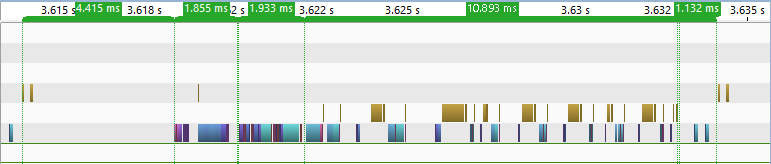
\includegraphics[width=1.0\textwidth]{TimelineSnapshot.png}
    \caption{Timeline overview of pipeline captured by NVIDIA Visual Profiler. Each colored block indicates a different kernel. The MemCpy rows indicate memory transfers between the device and host. The time periods delineated in green indicate the stages of the pipeline. From left to right: Memory Management, Preprocessing, Segmentation, Mesh Generation, and OpenGL Visualization}
    \label{fig:fulltimeline}
\end{figure}


\begin{figure}[!htpb]
    \centering
    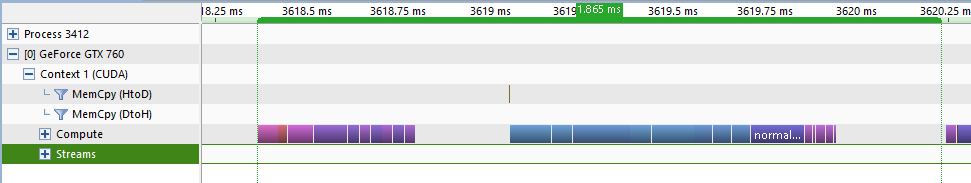
\includegraphics[width=1.0\textwidth]{PreprocessingTimeline.png}
    \caption{Timeline of the preprocessing stage of the pipeline captured by NVIDIA Visual Profiler. Each colored block indicates a different kernel. The MemCpy rows indicate memory transfers between the device and host.}
    \label{fig:preprocessingtimeline}
\end{figure}


\begin{figure}[!htpb]
    \centering
    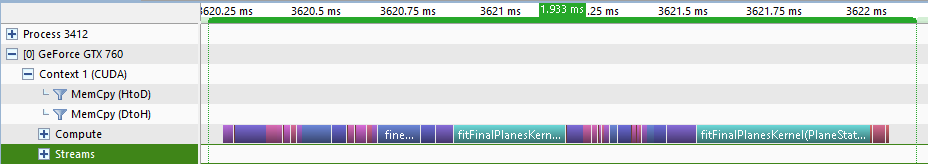
\includegraphics[width=1.0\textwidth]{SegmentationTimeline.png}
    \caption{Timeline of the segmentation stage of the pipeline captured by NVIDIA Visual Profiler. Each colored block indicates a different kernel. The MemCpy rows indicate memory transfers between the device and host.}
    \label{fig:segmentationtimeline}
\end{figure}

\begin{figure}[!htpb]
    \centering
    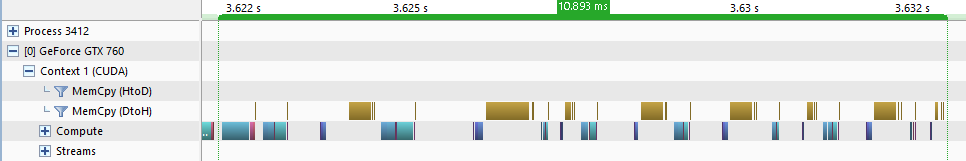
\includegraphics[width=1.0\textwidth]{MeshGenerationTimeline.png}
    \caption{Timeline of the mesh generation stage of the pipeline captured by NVIDIA Visual Profiler. Each colored block indicates a different kernel. The MemCpy rows indicate memory transfers between the device and host.}
    \label{fig:meshgenerationtimeline}
\end{figure}

\section{Normal Estimation Accuracy}
\begin{figure}[!htpb]
    \centering
    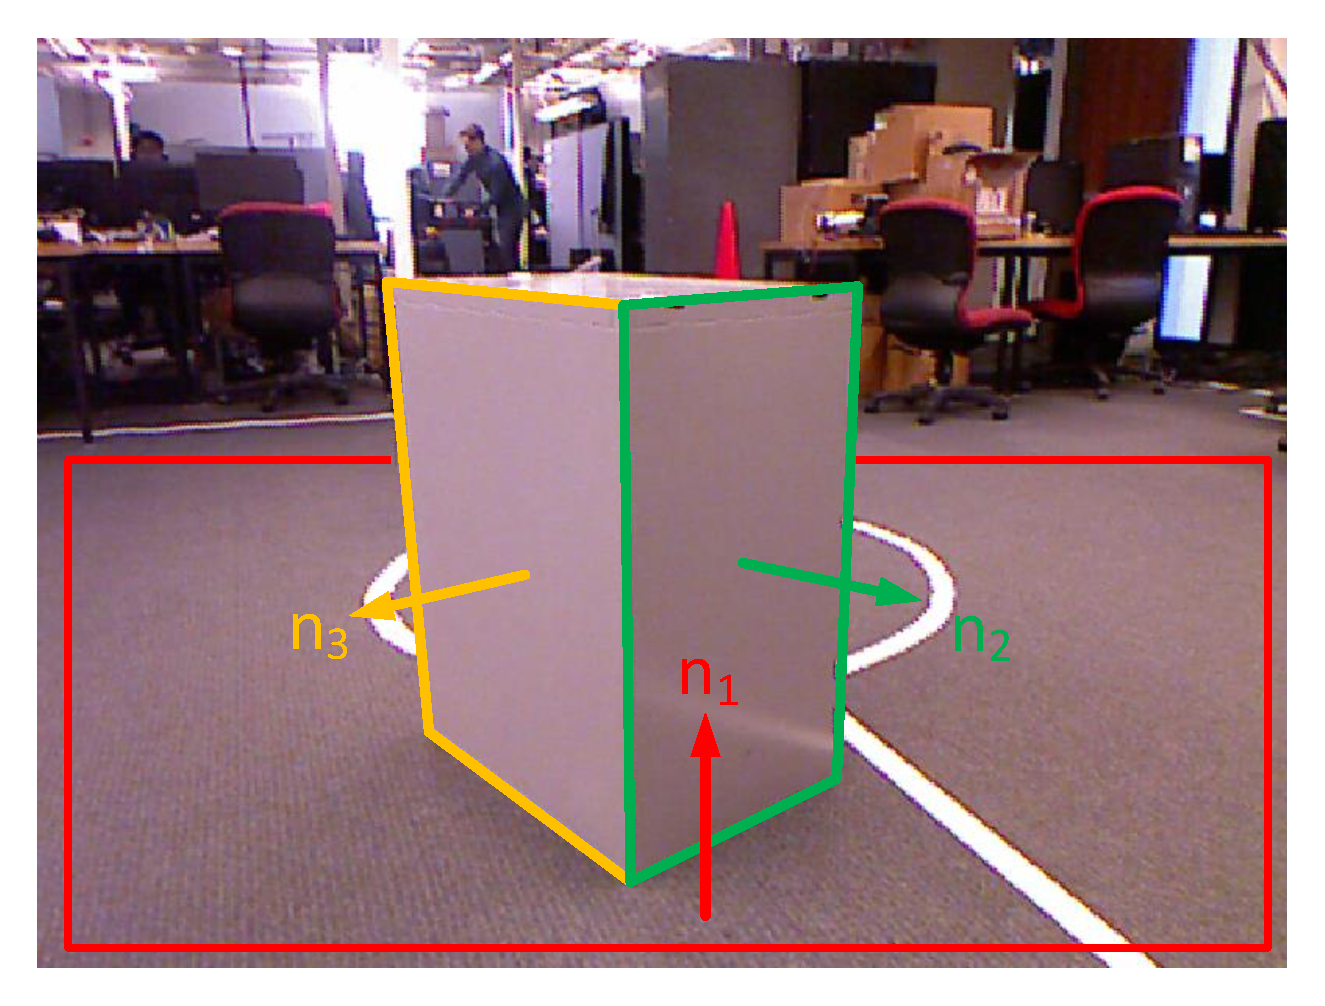
\includegraphics[width=0.7\textwidth]{BoxNormalsDrawing.pdf}
    \caption{Normal accuracy analysis test set with true planes and normals drawn on top.}
    \label{fig:boxnormalsdrawing}
\end{figure}
To assess the accuracy of the point normal estimation system, two different metrics were applied to the test set in Figure~\ref{fig:boxnormalsdrawing}. First, the normals of the three planes generated by the pipeline ($\vec{n_1},\vec{n_2},\vec{n_3}$) should should be perfectly orthogonal. By measuring the angle between the vectors pairwise, we have a good surrogate metric for the accuracy of the plane fits. Table~\ref{table:orthonormalerror} shows the relative error between each pair of vectors. The largest error is between  $\vec{n_2}$  and $\vec{n_3}$, and even then it's only $1.443^{\circ}$.
\begin{table}[h]
\label{table:orthonormalerror}
\begin{tabular}{|l|l|l|}
\hline
Vector pair                             & Angle between vectors            & Error from orthogonal           \\ \hline
$\cos^{-1}(\vec{n_1} \cdot  \vec{n_2})$ & $89.274^{\circ}$ & $0.726^{\circ}$ \\ \hline
$\cos^{-1}(\vec{n_1} \cdot  \vec{n_3})$ & $89.955^{\circ}$ & $0.045^{\circ}$ \\ \hline
$\cos^{-1}(\vec{n_2} \cdot  \vec{n_3})$ & $88.557^{\circ}$ & $1.443^{\circ}$ \\ \hline
\end{tabular}
\end{table}

The second metric is to measure each segmented point's local normal with the final plane normal estimated by the pipeline. Figure~\ref{fig:normalheatmap} shows several heat maps of this error metric for the various depth filters and normal estimation methods. With the simple normal estimator and no depth filtering, the pipeline completely fails, so no data is available for that combination. Clearly the normal averaging has a significant effect on the normal error. Also, the largest errors tend to occur around sharp edges, which is to be expected.

\begin{figure}[!htpb]
    \centering
    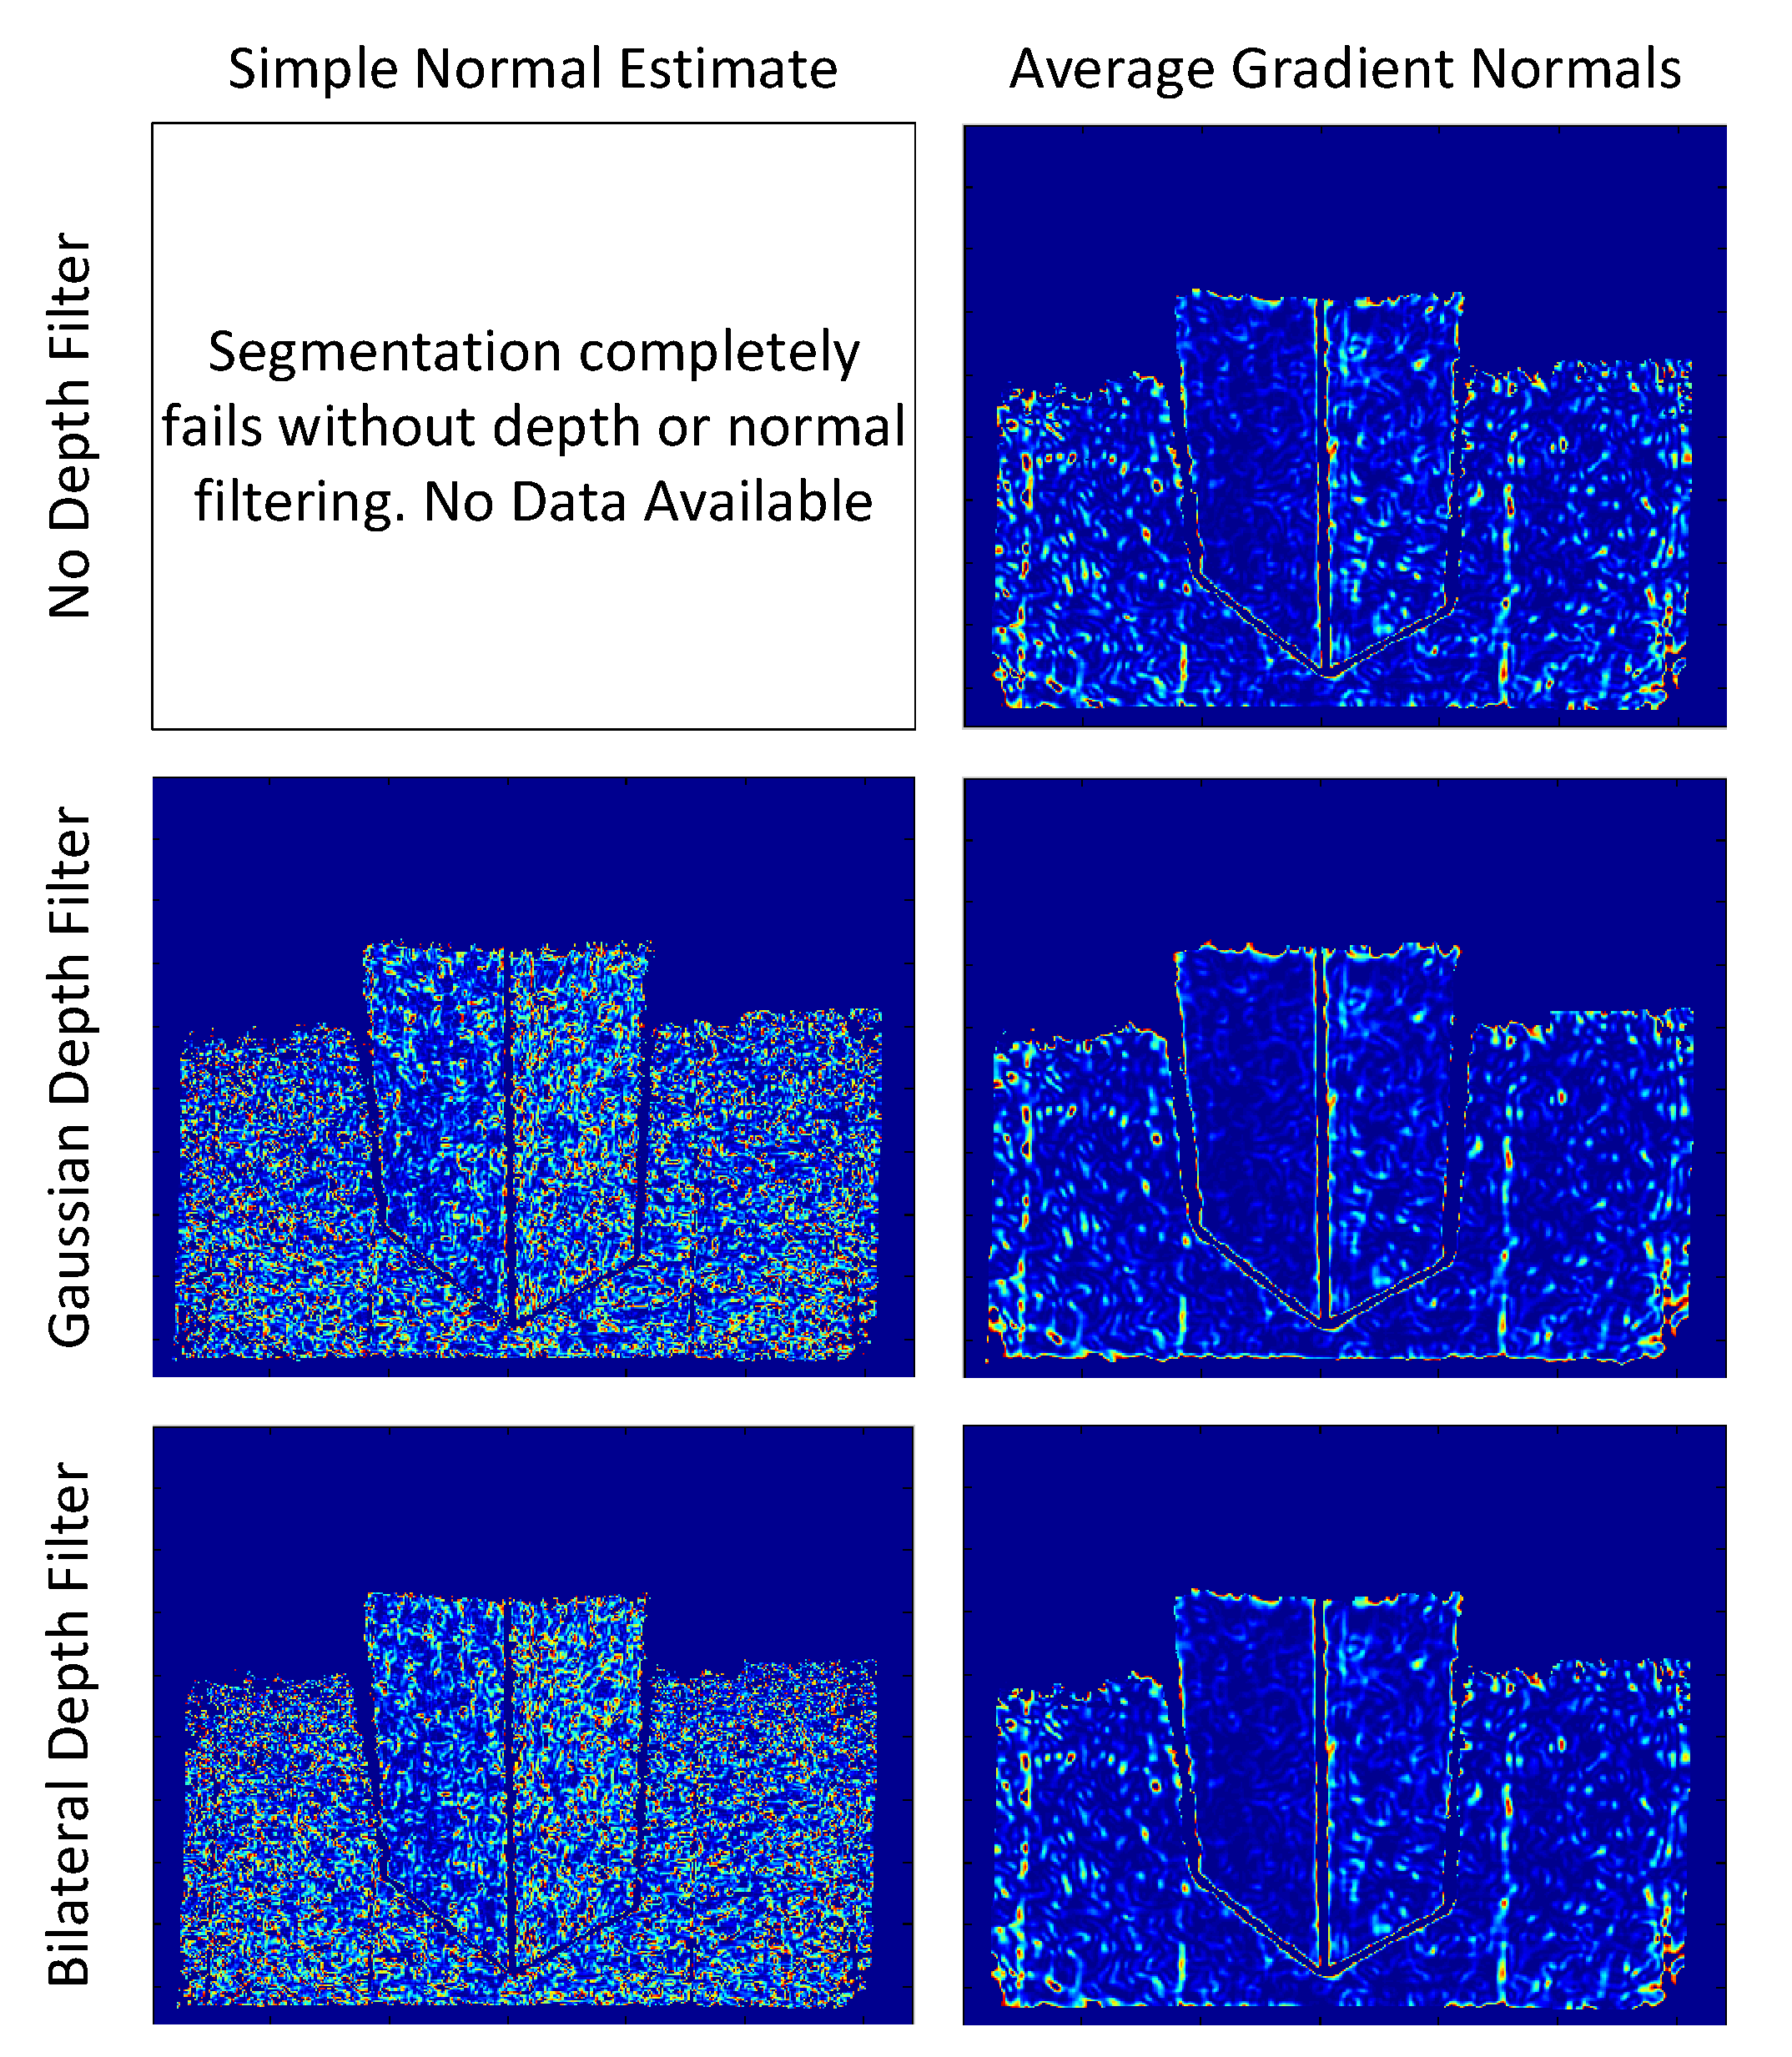
\includegraphics[width=0.7\textwidth]{NormalErrorHeatmap.pdf}
    \caption{Heat map of local normal estimation errors compared to the found planes for various filters and estimation techniques. Values range from $0^{\circ}$ off-angle (dark blue) to $2^{\circ}$ off-angle (bright red). Unsegmented pixels appear as dark blue.}
    \label{fig:normalheatmap}
\end{figure}

\section{QuadTree Efficiency}
\begin{figure}[!htpb]
    \centering
    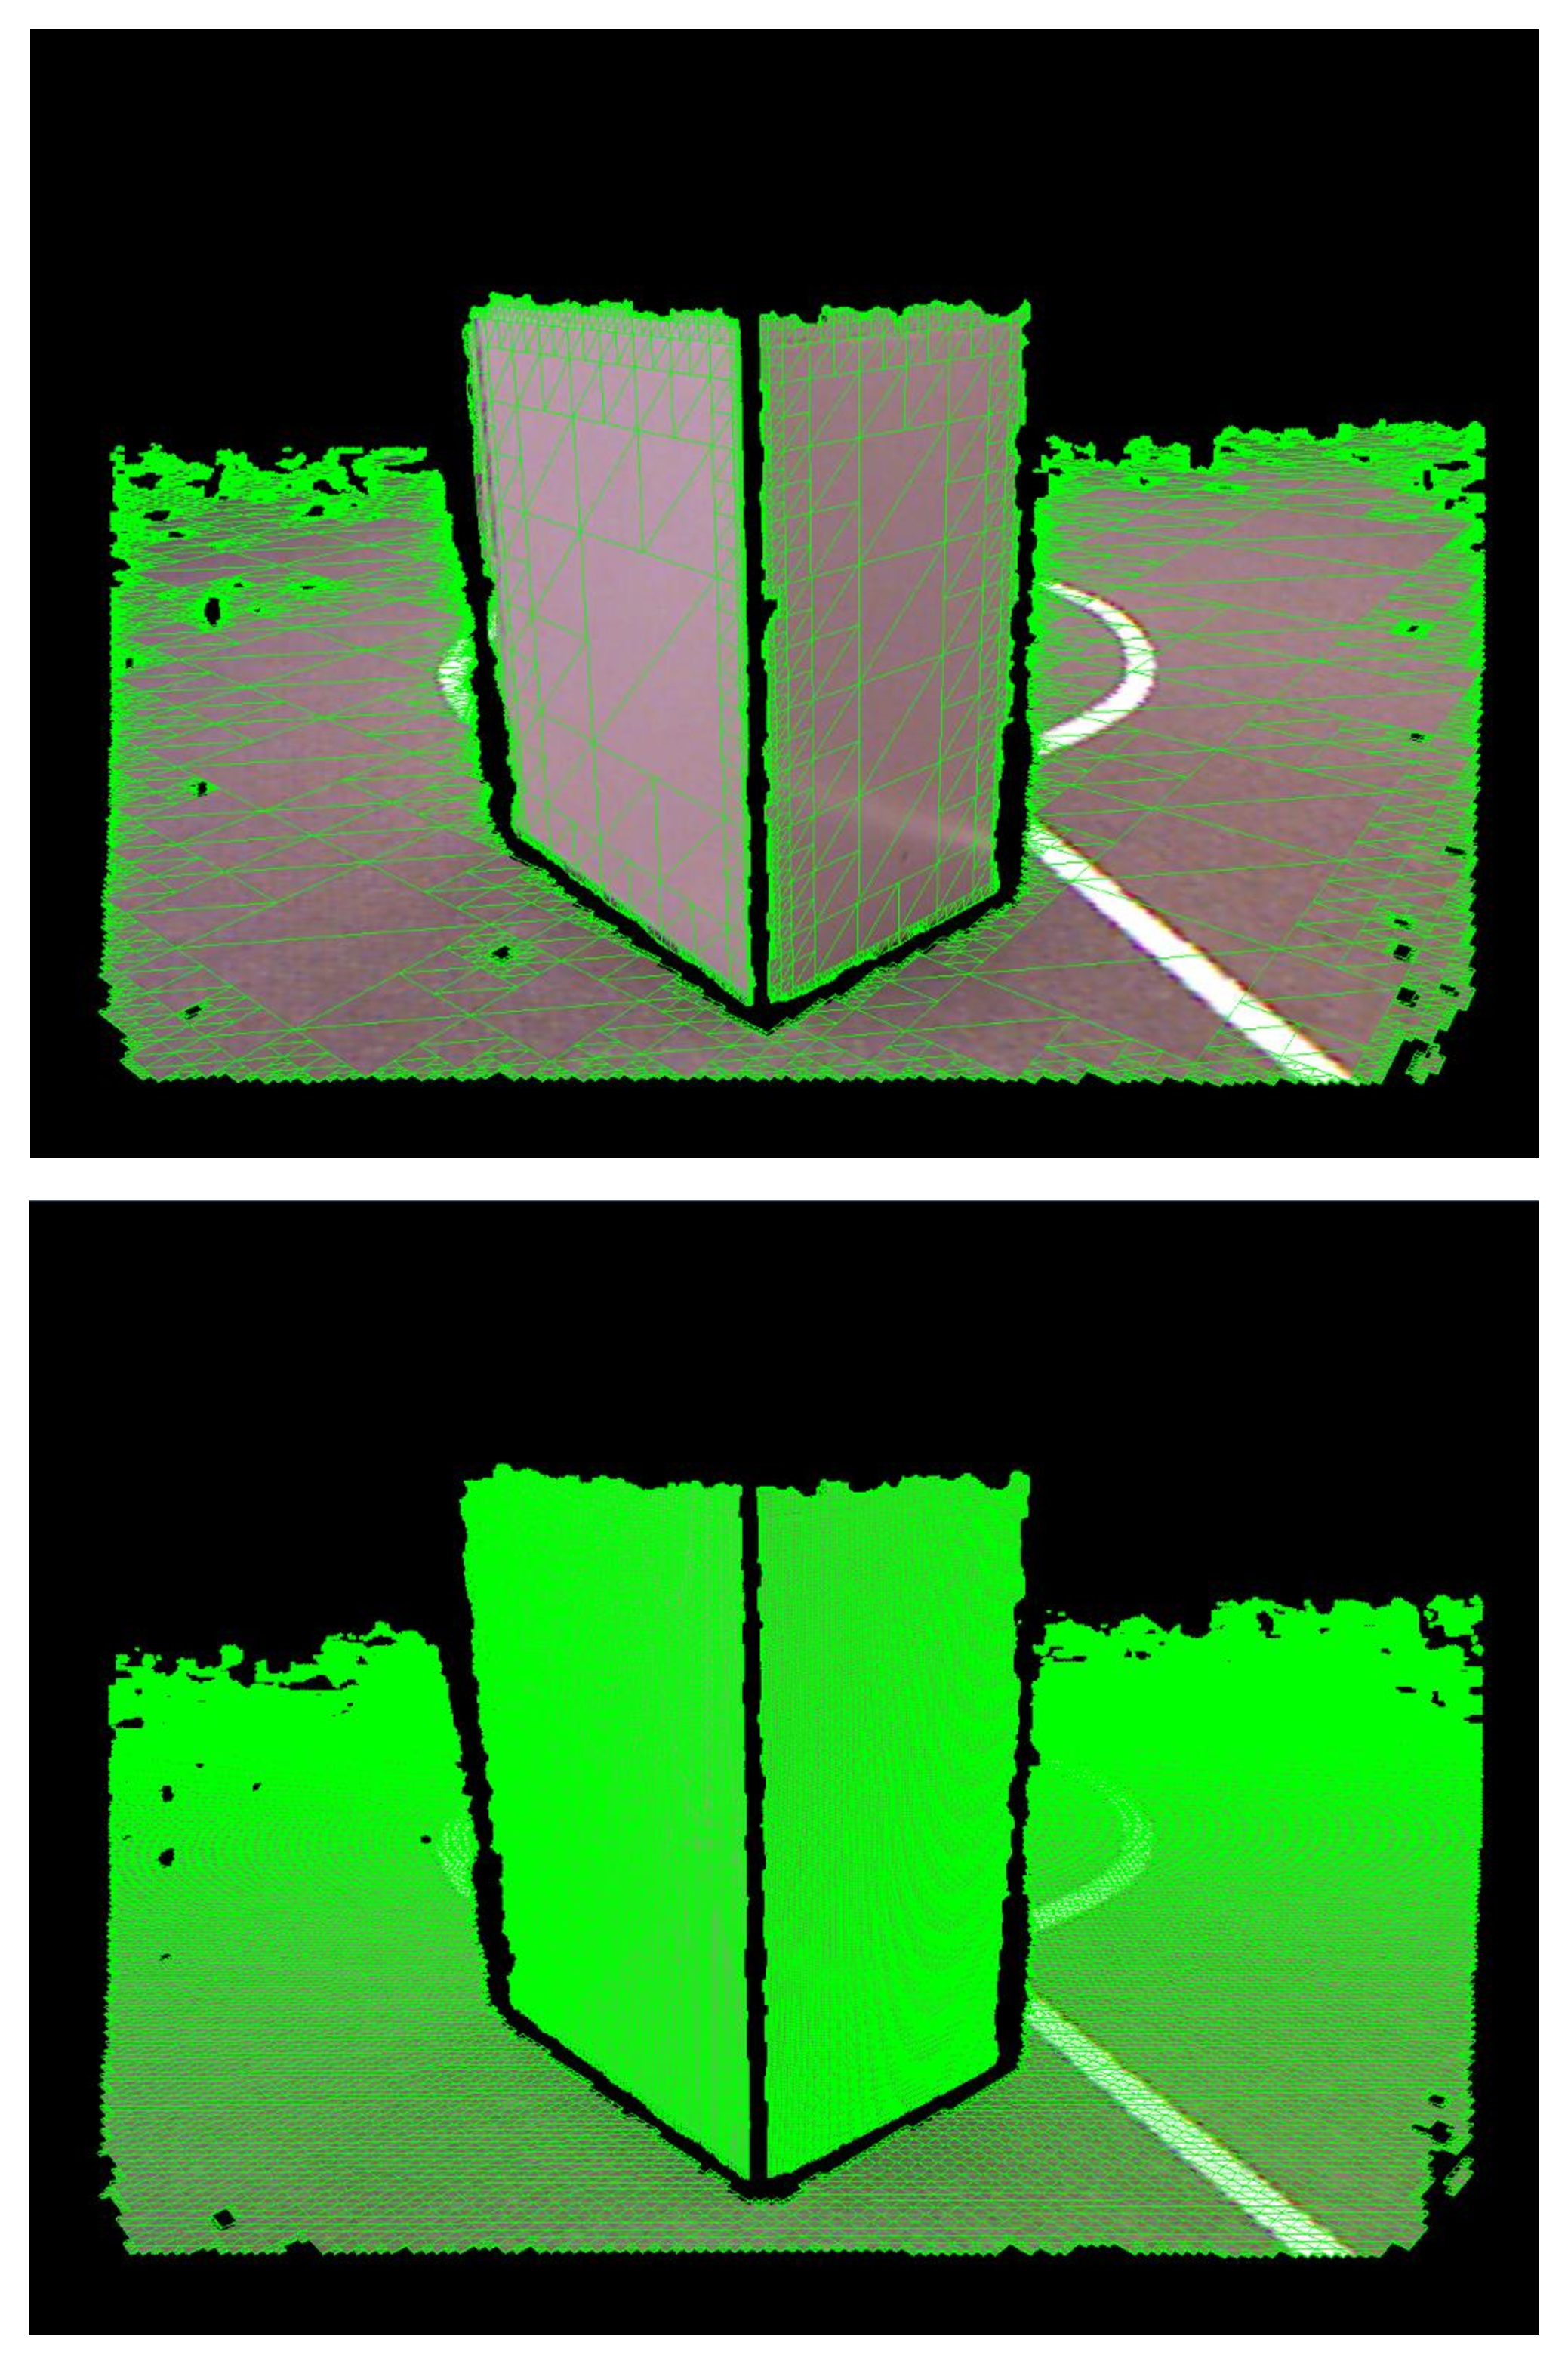
\includegraphics[width=0.9\textwidth]{BoxWithAndWithoutQuadTree.pdf}
    \caption{Comparison of textured mesh generated with (top, 76,698 vertices) and without (bottom, 18,573 vertices) QuadTree optimization.}
    \label{fig:withwithoutquadtree}
\end{figure}
The effectiveness of the QuadTree mesh simplification algorithm is difficult to measure fairly, since it was designed to optimize memory storage over multiple frames not frame by frame. So first, I will offer an apples to apples comparison between a set of meshes generated with and without QuadTree decimation on the same dataset. Figure~\ref{fig:withwithoutquadtree} shows a visual comparison of the triangulations. The original mesh consists of 76,698 vertices. The simplified QuadTree mesh uses only 18,573 vertices, roughly 25\% of the original mesh size.\par
However, the space these figures are computed in is a projection of the original image into a flat space. Depending on the size of the plane in the image, this space may be downscaled or upscaled to fit the texture efficiently. To show the practical effect this has on compression ratio, Figure~\ref{fig:compressionratio} compares the measured compression ratio for multiple scenes plotted against the number of planar points in the original image. Note that only for some very small planes does the ratio go above 1, and for most they are at or below 0.25.  This suggests that even if the mesh had been generated in camera space with a greedy meshing algorithm, the QuadTree representation would still be more space efficient in representing the geometry.\par
In addition, because the QuadTrees are restricted to a plane, each vertex only requires 2 degrees of freedom, whereas the greedy camera space triangulation requires 3 per vertex. Therefore, the storage requirements of the QuadTree are reduced by roughly another third over an equivalent 3D free mesh.\par 


\begin{figure}[!htpb]
    \centering
    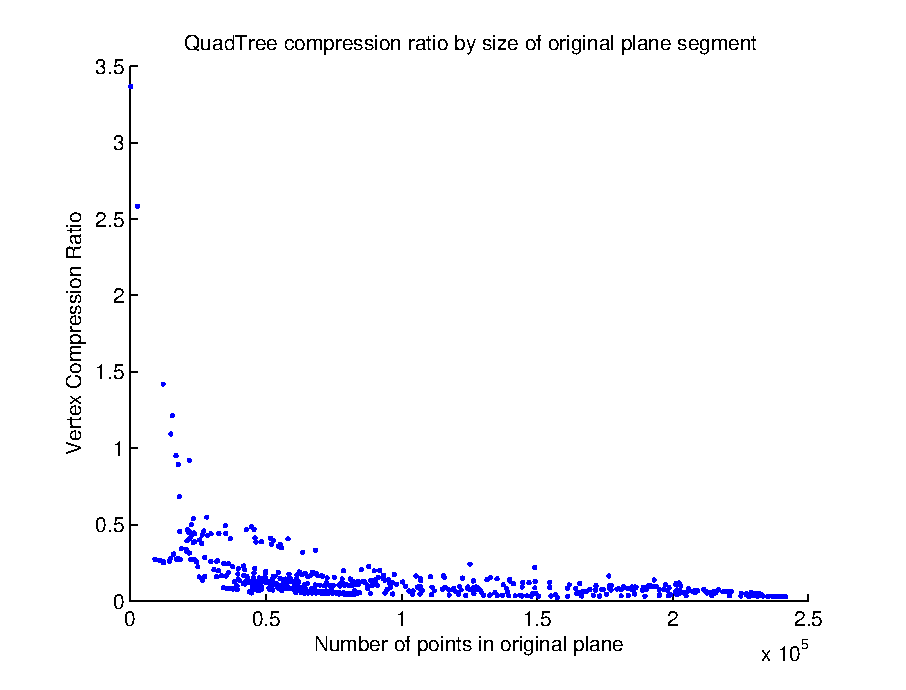
\includegraphics[width=0.9\textwidth]{CompressionRatio.eps}
    \caption{QuadTree vertex compression ratio measured for many different scenes. Compression is measured as number of pixels in the original plane segment over number of vertices in the final mesh.}
    \label{fig:compressionratio}
\end{figure}



\begin{figure}[!htpb]
    \centering
    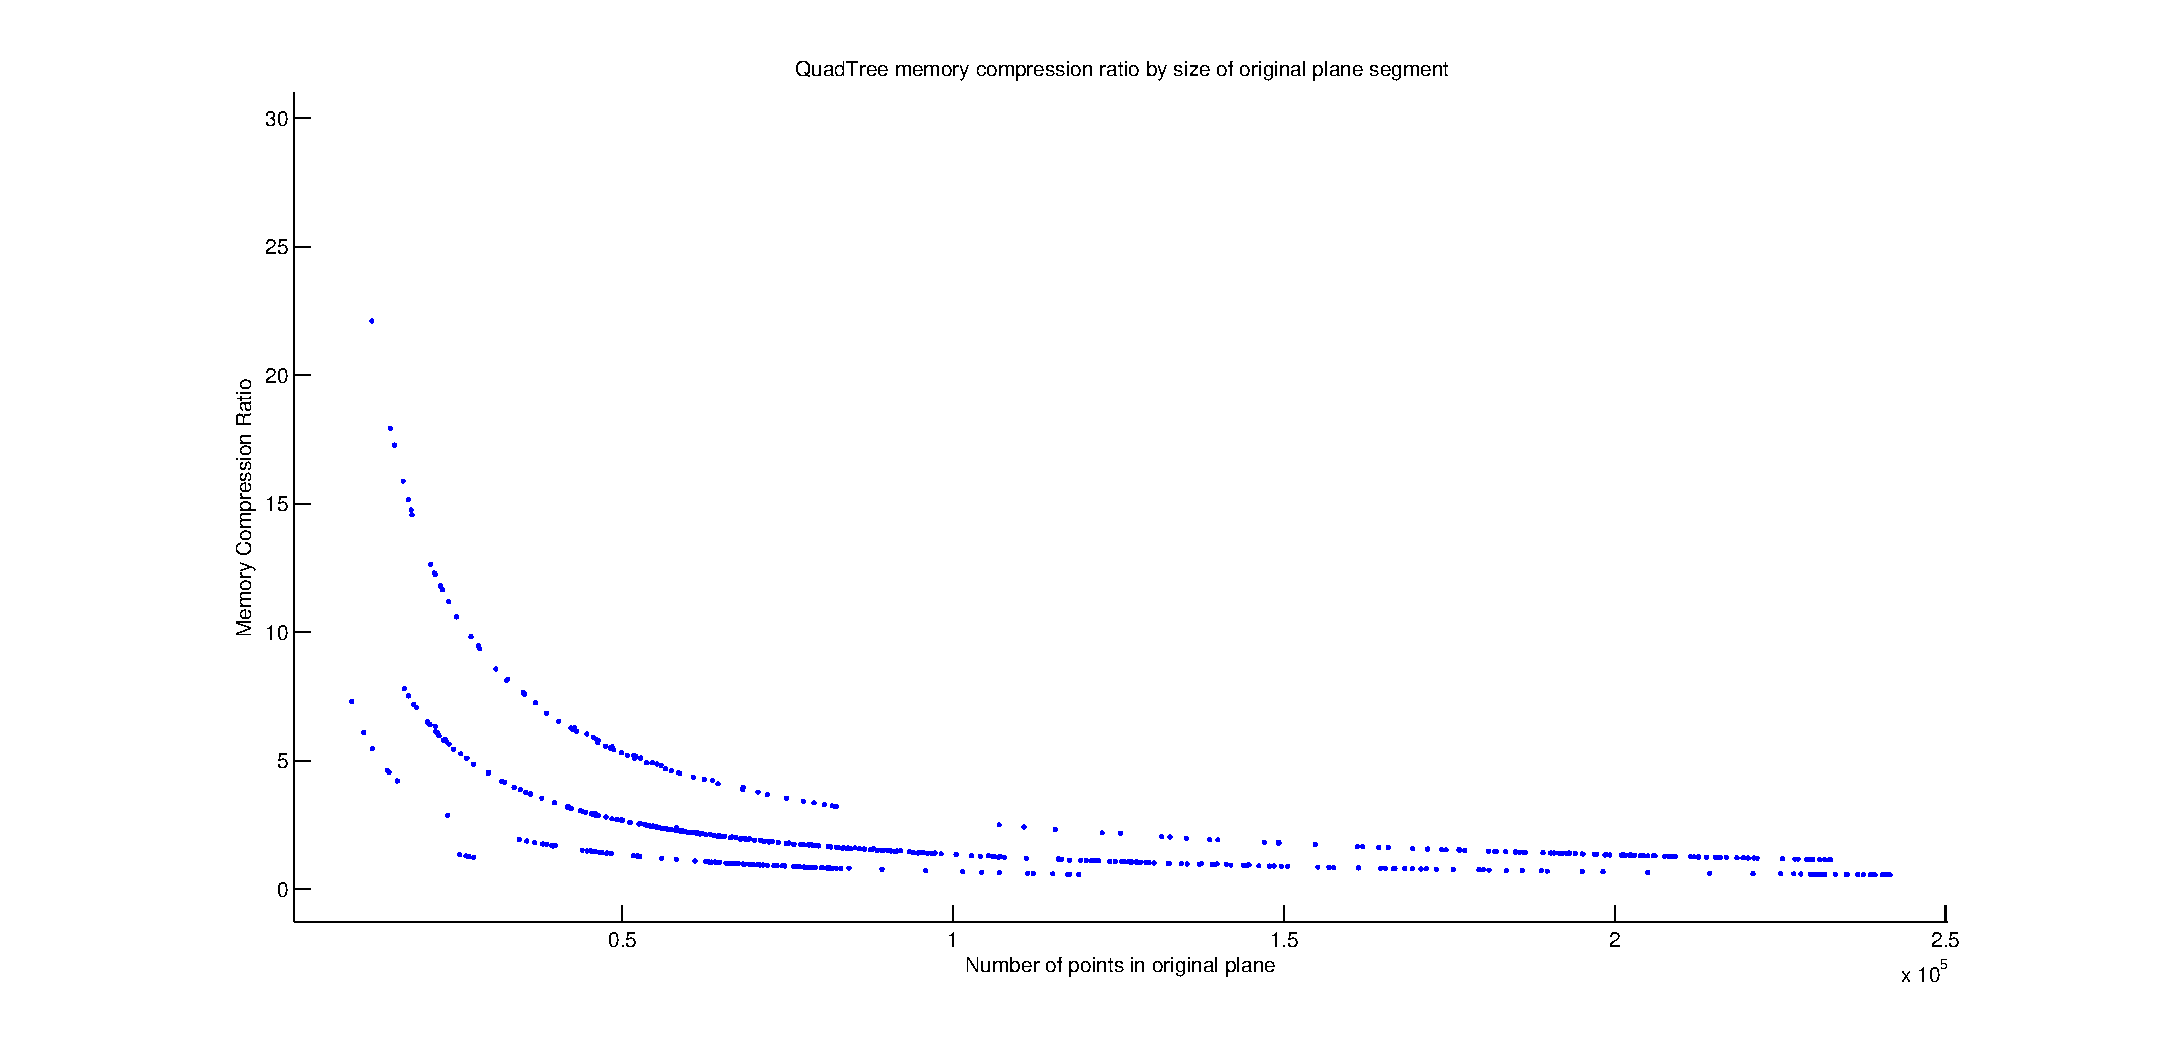
\includegraphics[width=0.9\textwidth]{MemoryCompressionRatio.eps}
    \caption{QuadTree total memory compression ratio measured for many different scenes. Compression is measured as number of bytes required by quadtree+color texture over number of bytes required by greedy triangulation with vertex coloring.}
    \label{fig:memorycompressionratio}
\end{figure}

However, adding in the color texture representation results in a net gain in memory usage due to the higher resolution offered by the texture. Also, texture dimensions are fixed to be powers of 2, so many textures are larger than their contents. Figure~\ref{fig:memorycompressionratio} shows the theoretical memory usage for the same data set as Figure~\ref{fig:compressionratio}. Because of this up-sampling and because the segments are projected into textures the size of their bounding box, a lot of the texture space is underutilized. Note the distinct curves that emerge from the data due to the rounding up of texture dimensions to powers of two.\par 
So, the conclusion to draw from this data is that the memory savings from storing the mesh geometry in the QuadTree structure are quite significant, but at least for a single frame of data, including color information imposes a hefty additional memory burden. The hope is that as new frames are collected and integrated, this additional memory will be reused and the new color information will be trivial to integrate with the preexisting texture.